% Made up for the tikra benchmark.
\usetikzlibrary{mindmap}
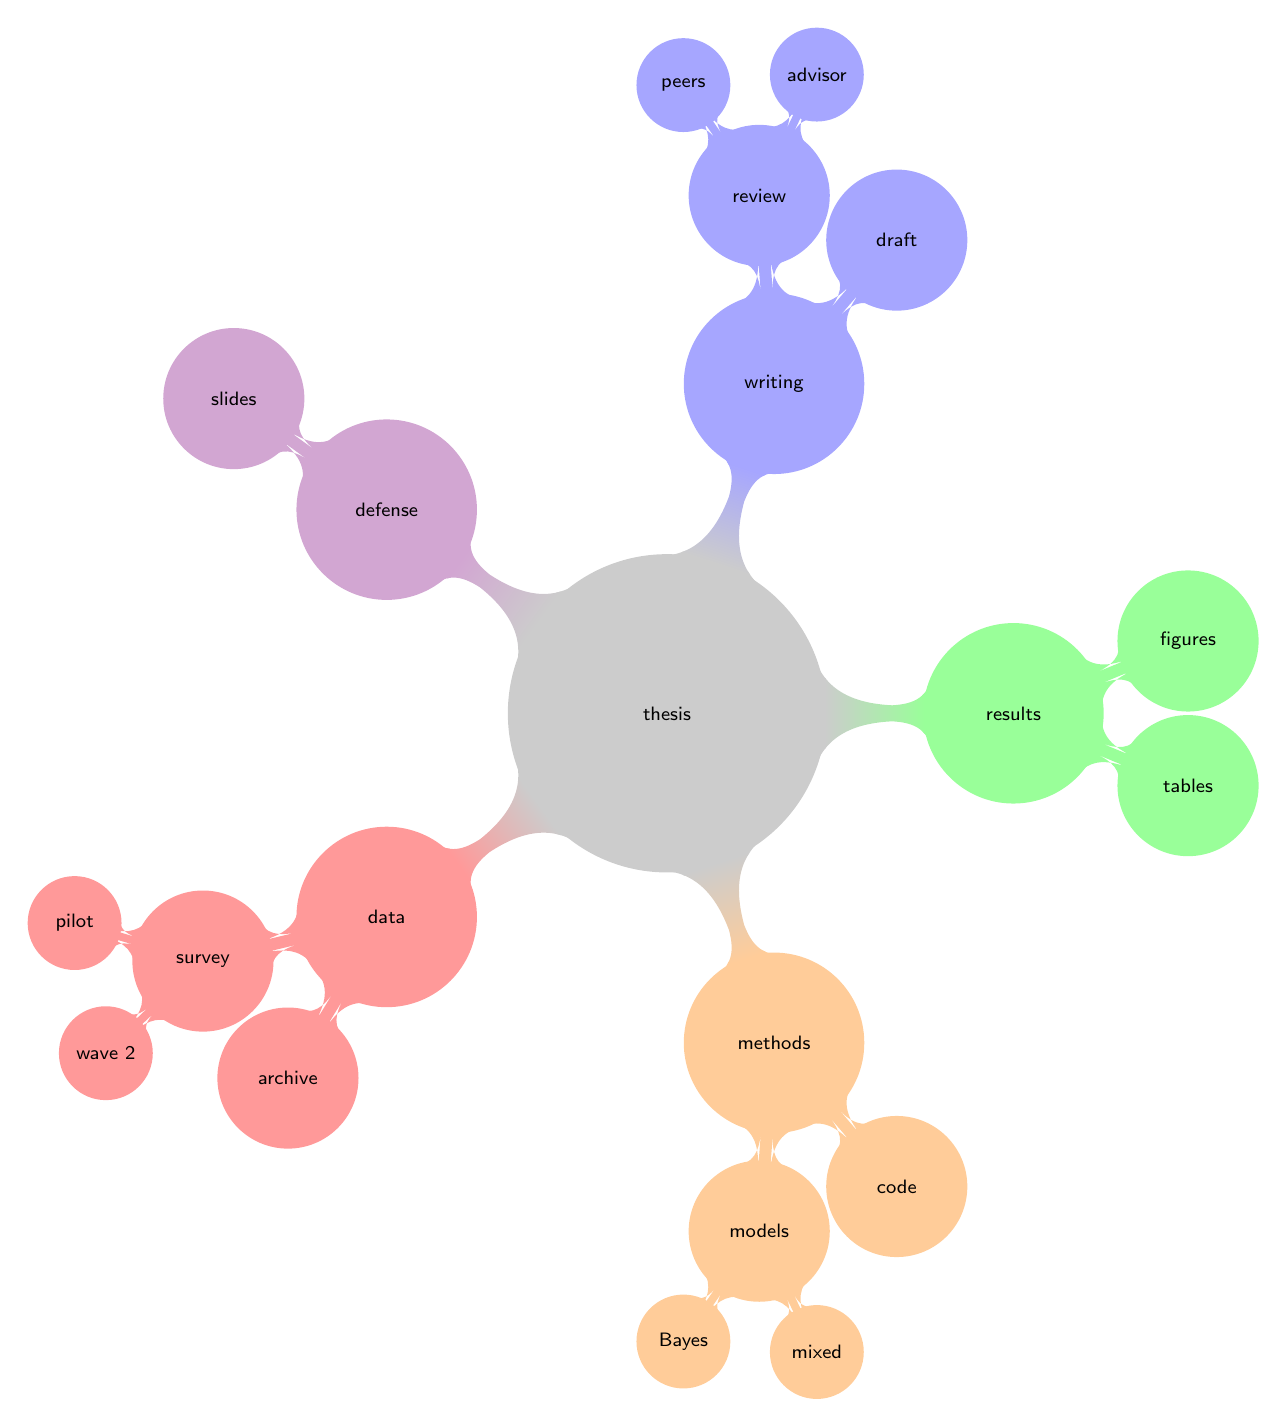
\begin{tikzpicture}[mindmap, grow cyclic, every node/.style={concept, font=\sffamily\scriptsize}, concept color=black!20, text=black,
    level 1/.append style={level distance=4.4cm, sibling angle=72},
    level 2/.append style={level distance=2.4cm, sibling angle=45},
    level 3/.append style={level distance=1.7cm, sibling angle=60}]
  \node {thesis}
    child[concept color=red!40] { node {data}
      child { node {survey} child { node {pilot} } child { node {wave 2} } }
      child { node {archive} } }
    child[concept color=orange!40] { node {methods}
      child { node {models} child { node {Bayes} } child { node {mixed} } }
      child { node {code} } }
    child[concept color=green!40] { node {results}
      child { node {tables} }
      child { node {figures} } }
    child[concept color=blue!35] { node {writing}
      child { node {draft} }
      child { node {review} child { node {advisor} } child { node {peers} } } }
    child[concept color=violet!35] { node {defense}
      child { node {slides} } };
\end{tikzpicture}
